\chapter{Conclusions and Intended Work}
\label{chp:4}
In this report, I have provided a brief overview of current theories on the
development of AD, an introduction to the family of models used to model AD on
brain networks and inference methods for comparing these with data. In this
final chapter, I will outline my research objectives and intended future work,
before offering some concluding remarks. 

Over the next year, I intend to work on incorporating additional features of AD 
pathology into the modelling framework presented here. There are two targets of 
interest, \AB and genetic risk factors such as APOE4. I will also continue 
to develop software facilitating modelling and inference for macro-scale 
brain modelling. I will briefly outline the intended scope of these projects. 

\section{\TP and \AB interactions}

The task of producing a full model of proteopathy remains an open challenge in 
AD research. In \cref{chp:3} we described a fully generative model of  
\TP PET data that is capable of describing our observations across the AD
progression timeline with great accuracy. Our results highlight that there are
dynamical changes to \TP occurring throughout the disease trajectory, namely \TP
proteopathy is diffusion dominated in early AD and becomes growth dominated in
late AD. Since the model only addresses the dynamics of \TP, we are limited in
how we can interrogate these dynamical shifts. Decades of research, including
through brain imaging such as PET, indicate that the single largest
co-conspirator along with \TP is \AB
\cite{pooler2015,bennett2017enhanced,he2018amyloid,ossenkoppele2022amyloid}. The
wealth of evidence toward \AB involvement and the available data makes it a
prime target for mathematical models and probabilistic inference. 

We have already presented a mathematical kinetic model of \TP and \AB interaction 
in \cite{thompson2020}. The model presented is a coupled pair of heterodimer 
models, four equations in total, with two describing healthy and toxic \AB and 
another two describing healthy and toxic \TP. The model is: 

\begin{subequations}
    \label{eqn:conspiracy-model}
    \begin{alignat}{3}
        \odl{u_i}{t} &= -\rho \lap{u_j} + a_0  &&- a_1 u_i - a_2 u_i \tilde{u}_i 
        \label{eqn:conspiracy-model-healthyAB} \\ 
        \odl{\tilde{u_i}}{t} &= -\tilde{\rho} \lap{\tilde{u}_j} &&- \tilde{a}_1 \tilde{u}_i + a_2 u_i \tilde{u}_i 
        \label{eqn:conspiracy-model-toxicAB} \\ 
        \odl{v_i}{t} &= -\sigma \lap{v_j} + b_0 &&- b_1 v_i - b_2 v_i \tilde{v}_i - b_3 \tilde{u}_i v_i \tilde{v}_i 
        \label{eqn:conspiracy-model-healthyTP} \\ 
        \odl{\tilde{v_i}}{t} &= -\tilde{\sigma} \lap{\tilde{v}_j}  &&-\tilde{b}_1 v_i + b_2 v_i \tilde{v}_i + b_3 \tilde{u}_i v_i \tilde{v}_i,
        \label{eqn:conspiracy-model-toxicTP}
    \end{alignat}
\end{subequations}
where, $u$ and $\tilde{u}$ represent healthy and toxic \AB, respectively, and
$v$ and $\tilde{v}$ represent healthy and toxic \TP, respectively. The model is
identical to two heterodimer models \cref{eqn:network-heterodimer}, with an
additional interaction term between \cref{eqn:conspiracy-model-healthyTP} and
\cref{eqn:conspiracy-model-toxicTP}, $\pm b_3 \tilde{u}_i v_i \tilde{v}_i$. 
The interaction term describes an acceleration of toxic \TP induced
conformational changes to healthy \TP due to the presence of toxic \AB. This 
results in an acceleration of \TP accumulation when it is co-localised with \TP, 
providing a possible mechanism for explaining the results presented in \cref{chp:3}. However, the model is too complicated to be calibrated with the 
data we have available, i.e. toxic \AB and \TP PET. In upcoming work, we intend 
to build on models developed in \cite{kevrekidis2020anisotropic}, who present 
a linearisation of \cref{eqn:conspiracy-model} similar to that presented in 
\cref{sec:model-reduction-fkpp}, to make the \cref{eqn:conspiracy-model}
identifiable given the available data.

\section{Genetic Risk Factors}

AD is a highly heritable disease, with the strongest genetic risk coming from
apolipoprotein E-4 (APOE4) allele of the APOE gene \cite{corder1993gene,
lambert2013meta}. The APOE4 gene has been shown to accelerate both \AB and \TP
proteinopathies and brain atrophy \cite{liu2017apoe4, shi2017apoe4}. APOE4 has
been shown to possess many functions, including to facilitate neuronal growth,
signalling, the aggregation or clearance of \AB and the regulation of neuronal
myelination \cite{hunsberger2019role, kanekiyo2014apoe, blanchard2022apoe4}.
However, the exact mechanisms through which APOE4 contributes to AD remain
unclear. We hope to address the mechanistic action of APOE4 using the modelling
and inference framework presented throughout this work. Once we have a reliable
model of proteopathy in humans with AD, we will investigate how APOE4 acts on
model parameters to accelerate AD pathology. In the first instance, we plan to
do this using a cohort analysis, such as in \cref{chp:3}, to assess which
kinetic parameters are affected by the APOE4 genotype.

\section{Software Pipeline}
\label{sec:5-software}

The third project is an effort to make applying modelling and inference methods
to a relatively novel domain -- macroscale modelling and inference for
neurodegenerative disease -- easier, faster and more reproducible. At present,
there are a number of cumbersome steps in the modelling pipeline, including the
handling of patient data, generating and using the graph Laplacian and efficient
simulation of ODE models. Throughout my thesis I have made substantial use of
free and open source software to address these issues, in particular, packages
from the Julia programming language \cite{bezanson2012julia}, such as
DifferentialEquations.jl \cite{rackauckas2017differentialequations}, Turing.jl
\cite{tarek2020dynamicppl} and Makie.jl \cite{DanischKrumbiegel2021}. During my
DPhil, I have been developing Connectomes.jl
(\url{https://github.com/PavanChaggar/Connectomes.jl}), a package for processing
connectivity matrices associated with parcellation data. At present, the package
has read and write functionality, interfaces with Graphs.jl
\cite{fairbanks2021juliagraphs} to make use of algorithms in graph theory and
Makie.jl \cite{DanischKrumbiegel2021} for connectome and parcellation
visualisation (used throughout this thesis). The next steps are: 1) to build a
light wrapper around the DifferentialEquations.jl
\cite{rackauckas2017differentialequations} package to specialise performance on
the numerical solutions to models on a connectome; 2) create an interface that
simplifies handling longitudinal patient data summarised on over a parcellation.
The combination of these additions will make it easier to model and also make it
easier to collaborate with other researchers. 

\section{Concluding Remarks} 
Insight into the mechanisms of AD in humans have typically been obtained using
animal or in-vitro studies that isolate component parts of AD. Being able to
garner useful mechanistic insights from in-vivo human patient data adds richness
and coherence to our current knowledge of AD. The combination of mathematical
modelling and human neuroimaging data provides a non-invasive method for
investigating AD pathology in humans. A major theme I have attempted to
communicate here is that marriage of dynamical systems modelling and human
neuroimaging data is achievable through Bayesian analysis. In \cref{chp:2}, I
described a family of graph based models and the problem of Bayesian inference.
In \cref{chp:3}, I showed that a physics based generative model of \TP is
identifiable and can be fit to patient data using MCMC methods, providing
biologically insight into differences in disease dynamics across cohorts. Going 
forward, it will be important to incorporate other covariates into our models of 
AD so that we can develop a complete theory of AD pathology.

\section{Thesis Outline}

In this section, I will overview my intended thesis and timetable for submission 
before Michaelmas term 2023. 

\begin{enumerate}
    \item Introduction \\
    In this chapter, I will overview the necessary background information that 
    presupposes the later chapters. In particular, I will provide a summary 
    of the biological underpinnings of AD and the brain imaging methods used 
    to make observations from humans in-vivo. I will also describe the current 
    approaches used within the literature for mathematical modelling of 
    neurodegenerative disorders. I will conclude with a thesis outline.
    \begin{enumerate}
        \item Motivation and Thesis Aims 
        \item Biological foundations of AD
        \item Neuroimaging of AD 
        \item Dynamical models of AD
        \item Thesis outline
    \end{enumerate}
    \item Model Development and Identifiability analysis \\ 
    In this chapter, I will describe the mathematical basis for the family of
    reaction diffusion models used throughout this work. This consists of two
    parts, a model of protein transport throughout the structural connectome and
    a local models of protein reaction dynamics. I will also present
    computational results on the identifiability of these reaction-diffusion
    equations on graphs given idealised data and real patient data. Parts of
    this chapter will be adapted from \cite{schafer2022correlating}.
    \begin{enumerate}
        \item Modelling aims
        \item Transport and structural connectivity
        \item Protein Proliferation: how toxic proteins accumulate
        \item Identifiability analysis of FKPP
        \item Application to AD
    \end{enumerate}
    \item Physics Based Generative Model of \TP \\
    This chapter will include the work presented in \cref{chp:3} and will follow
    a similar outline. I will first derive a local model of \TP proteopathy
    and describe how I estimate fixed parameters corresponding to regionally
    specific baseline values and growth rates. I will then apply this model to 
    patient data from ADNI and BioFINDER 2 data and discuss the results. A 
    manuscript for this work is currently being prepared for submission.
    \begin{enumerate}
        \item Motivation and Aims
        \item Deriving a local model of \TP pathology
        \item Estimating fixed regional parameters from data
        \item Inference using \TP PET data
        \item Discussion and conclusions
    \end{enumerate}
    \item Dynamical Model of proteopathy in AD: \AB and \TP interaction \\
    In this chapter I will describe our efforts to condense a model of \AB and
    \TP such that it can be calibrated against patient data. Once a
    coarse-grained model of \AB and \TP interaction has been developed, I intend
    to calibrate it with patient data from ADNI and BioFINDER 2. I anticipate
    that this will provide insight into the results obtained in \cref{chp:3} and
    elucidate the macroscale influence of \AB on \TP dynamics. Depending on the
    time taken to complete this work, I hope to add results on the effect
    of APOE4 on AD proteopathy into this work.
    \begin{enumerate}
        \item Motivation and Aims 
        \item Coarse graining a conspiracy theory
        \item Multimodal inference using \AB and \TP PET 
        \item Discussion and conclusions
    \end{enumerate}
    \item Concluding Remarks and Future Work
    In this chapter, I will briefly summarise the contributions of this thesis 
    and assess to what extent our aims are met. Based on this assessment and the 
    state of the field, I will suggest future avenues of research to extend the 
    work presented.
\end{enumerate}

My plans for submission can be seen in \cref{fig:stupid-gant-chart}

\begin{figure}[H]
    \centering
    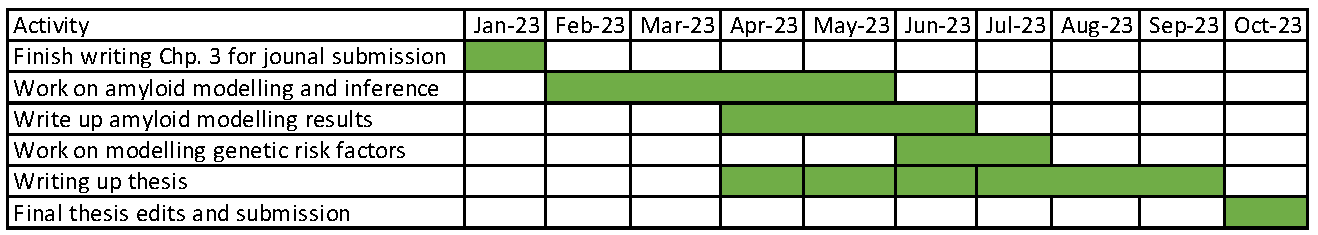
\includegraphics[width=1.0\textwidth]{gant.pdf}
    \caption{\textbf{Future work and submission timetable}}
    \label{fig:stupid-gant-chart}
\end{figure}